% This LaTeX document needs to be compiled with XeLaTeX.
\documentclass[
  10
]{article}
\usepackage[margin=2cm,includehead=true,includefoot=true,centering,]{geometry}
\usepackage{xcolor}
\usepackage{ucharclasses}
\usepackage{hyperref}
\usepackage{amsmath,amssymb}
\usepackage{amsfonts}
\usepackage[version=4]{mhchem}
\usepackage{stmaryrd}
\usepackage{bbold}
\usepackage{polyglossia}
\usepackage{fontspec}
\usepackage{ctex}
\usepackage[export]{adjustbox}
\usepackage{tabularx}
\usepackage{booktabs}

\usepackage{setspace}
\setstretch{1.2}

\makeatletter
\@ifundefined{KOMAClassName}{% if non-KOMA class
  \IfFileExists{parskip.sty}{%
    \usepackage{parskip}
  }{% else
    \setlength{\parindent}{0pt}
    \setlength{\parskip}{6pt plus 2pt minus 1pt}}
}{% if KOMA class
  \KOMAoptions{parskip=half}}
\makeatother
\usepackage{graphicx}
\makeatletter
\newsavebox\pandoc@box
\newcommand*\pandocbounded[1]{% scales image to fit in text height/width
  \sbox\pandoc@box{#1}%
  \Gscale@div\@tempa{\textheight}{\dimexpr\ht\pandoc@box+\dp\pandoc@box\relax}%
  \Gscale@div\@tempb{\linewidth}{\wd\pandoc@box}%
  \ifdim\@tempb\p@<\@tempa\p@\let\@tempa\@tempb\fi% select the smaller of both
  \ifdim\@tempa\p@<\p@\scalebox{\@tempa}{\usebox\pandoc@box}%
  \else\usebox{\pandoc@box}%
  \fi%
}
% Set default figure placement to htbp
\def\fps@figure{htbp}
\makeatother
\setlength{\emergencystretch}{3em} % prevent overfull lines
\providecommand{\tightlist}{%
  \setlength{\itemsep}{0pt}\setlength{\parskip}{0pt}}


\hypersetup{colorlinks=true, linkcolor=blue, filecolor=magenta, urlcolor=cyan,}
\urlstyle{same}

\usepackage{colortbl}
\definecolor{table-row-color}{HTML}{999999}
\definecolor{table-rule-color}{HTML}{999999}
%\arrayrulecolor{black!40}
\arrayrulecolor{table-rule-color}     % color of \toprule, \midrule, \bottomrule
\setlength{\aboverulesep}{0pt}
\setlength{\belowrulesep}{0pt}


\setotherlanguages{english}
\IfFontExistsTF{Source Han Serif CN}
{\newfontfamily\chinesefont{Source Han Serif CN}}
{\IfFontExistsTF{Noto Serif CJK SC}
  {\newfontfamily\chinesefont{Noto Serif CJK SC}}
  {\IfFontExistsTF{SimSun}
    {\newfontfamily\chinesefont{SimSun}}
    {\IfFontExistsTF{FangSong}
      {\newfontfamily\chinesefont{FangSong}}
      {\newfontfamily\chinesefont{Arial Unicode MS}}
}}}
\IfFontExistsTF{Times New Roman}
{\newfontfamily\englishfont{Times New Roman}}
{\IfFontExistsTF{Liberation Serif}
  {\newfontfamily\englishfont{Liberation Serif}}
  {\IfFontExistsTF{DejaVu Serif}
    {\newfontfamily\englishfont{DejaVu Serif}}
    {\newfontfamily\englishfont{Arial}}
}}


\author{}
\date{}

\begin{document}


\subsection{超声波声速的测量}\label{ux8d85ux58f0ux6ce2ux58f0ux901fux7684ux6d4bux91cf}

\subsection{一、实验目的：}\label{ux4e00ux5b9eux9a8cux76eeux7684}

\begin{enumerate}
\def\labelenumi{\arabic{enumi}.}
\item
  掌握超声波测声速的物理原理；
\item
  学习示波器和信号源的原理与应用；
\item
  学习测量空气中声速的两种方法，了解声波在空气中传播速度与气体状态参量关系。
\end{enumerate}

\subsection{二、实验仪器：}\label{ux4e8cux5b9eux9a8cux4eeaux5668}

声速测定仪、示波器等

\subsection{三、实验原理：}\label{ux4e09ux5b9eux9a8cux539fux7406}

\subsection{1.
声波在空气中的传播速度}\label{ux58f0ux6ce2ux5728ux7a7aux6c14ux4e2dux7684ux4f20ux64adux901fux5ea6}

在理想气体中的传播速度为 \(\nu = \sqrt { \gamma R T / \mu }\) ，其中，γ
和 μ 是气体的比热容比和摩尔质量，T
为绝对温度，R为普适气体常数。由上式可知，声速仅与气体的温度和性质有关，与声源的频率无关。

因此，在传播介质的温度为t ℃时，干燥空气的声速理论值可由如下公式计算：

\[
v = v _ {0} \sqrt {1 + \frac {t}{T _ {0}}} = v _ {0} \sqrt {1 + \frac {t}{2 7 3 . 1 5}} = 3 3 1. 5 + 0. 6 t (m / S)
\]

\subsection{2.
超声波与压电陶瓷换能器}\label{ux8d85ux58f0ux6ce2ux4e0eux538bux7535ux9676ux74f7ux6362ux80fdux5668}

频率20Hz-20kHz的机械振动在弹性介质中传播形成声波，高于20kHz称为超声波，超声波的传播速度就是声波的传播速度，而超声波具有波长短，易于定向发射等优点。声速实验所采用的声波频率一般都在
20～60kHz
之间，在此频率范围内，采用压电陶瓷换能器作为声波的发射器、接收器效果最佳。

\pandocbounded{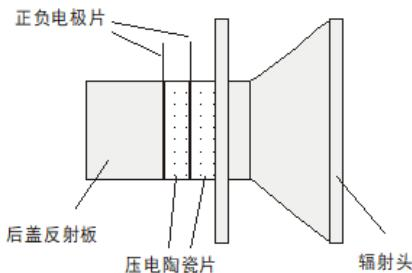
\includegraphics[keepaspectratio,alt={image}]{images/ca06f94364a76ccead32da1448b216de9a2c6f44d1f77c79bbe34f1fa72486d7.jpg}}

图1 纵向换能器的结构简图。

压电陶瓷换能器根据它的工作方式，分为纵向（振动）换能器、径向（振动）换能器及弯曲振动换能器。声速教学实验中所用的大多数采用纵向换能器。图
1为纵向换能器的结构简图。

\subsection{3.
共振干涉法（驻波法）测量声速}\label{ux5171ux632fux5e72ux6d89ux6cd5ux9a7bux6ce2ux6cd5ux6d4bux91cfux58f0ux901f}

假设在无限声场中，仅有一个点声源
S1（发射换能器）和一个接收平面（接收换能器S2）。当点声源发出声波后，在此声场中只有一个反射面（即接收换能器平面），并且只产生一次反射。

在上述假设条件下，发射波
\(\boldsymbol { \xi } _ { \ 1 } { = } \mathbf { A } _ { 1 } { \cos } ( \omega \mathrm { t } { - } 2 \pi \mathrm { x } / \lambda )\)
将在 S2处产生反射，反射波信号相位与\(\xi _ { 1 }\) 相反，即
\(\scriptstyle \xi _ { 2 } = \mathbf { A } _ { 2 } \mathbf { c o s } ( \mathbf { \omega } \mathbf { { t } } + 2 \pi \mathbf { x } / \lambda )\)
，幅度
\(\mathbf { A } _ { 2 } { < } \mathbf { A } _ { 1 } \circ \mathbf { \zeta } \boldsymbol { \xi } _ { 1 }\)
与 \(\xi _ { 2 }\) 在反射平面相交叠加，合成波束 \(\xi _ { 3 }\)

\[
\begin{array}{r l} \xi_ {3} & = \xi_ {1} + \xi_ {2} = A _ {1} \cos (\omega t - 2 \pi x / \lambda) + A _ {2} \cos (\omega t + 2 \pi x / \lambda) \\ & = A _ {1} \cos (\omega t + 2 \pi x / \lambda) + A _ {1} \cos (\omega t - 2 \pi x / \lambda) + (A _ {2} - A _ {1}) \cos (\omega t + 2 \pi x / \lambda) \\ & = 2 A _ {1} \cos (2 \pi x / \lambda) \cos \omega t + (A _ {2} - A _ {1}) \cos (\omega t - 2 \pi x / \lambda) \end{array}
\]

由此可见，合成后的波束 \(\xi _ { 3 }\) 在幅度上，具有随
cos(2πx/λ)呈周期变化的特性，在相位上，具有随(2πx/λ)呈周期变化的特性。另外，由于反射波幅度小于发射波，合成波的幅度即使在波节处也不为
0，而是按
\(( \mathbf { A } _ { 2 } \mathbf { \partial } - \mathbf { A } _ { 1 } ) \mathbf { c o s } ( \mathbf { \omega } \mathbf { \omega } \mathbf { \omega } + 2 \pi \mathbf { x } / \lambda )\)
变化。图 2
所示波形显示了叠加后的声波幅度，随距离按cos(2πx/λ)变化的特征。

\pandocbounded{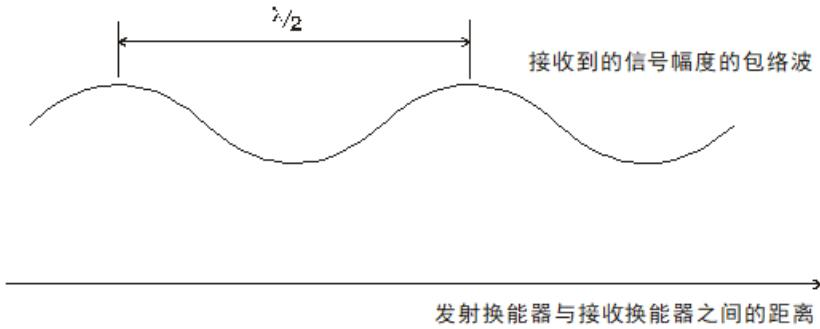
\includegraphics[keepaspectratio,alt={image}]{images/9f34e653b895666784278c948ddc3e74cfa1bdcb2e0c0c9e96203787758a27f8.jpg}}

图2 换能器间距与合成幅度

实验装置按图 所示，图中 和 为压电陶瓷换能器。
作为声波发射器，它由信号源供给频率为数十千赫的交流电信号，由逆压电效应发出一平面超声波；而
则作为声波的接收器，压电效应将接收到的声压转换成电信号。将它输入示波器，我们就可看到一组由声压信号产生的正弦波形。由于S2在接收声波的同时还能反射一部分超声波，接收的声波、发射的声波振幅虽有差异，但二者周期相同且在同一线上沿相反方向传播，二者在和S2区域内产生了波的干涉，形成驻波。我们在示波器上观察到的实际上是这两个相干波合成后在声波接收器
S2处的振动情况。移动S2
位置（即改变S1和S2之间的距离），从示波器显示上会发现，当
在某此位置时振幅有最大值。根据波的干涉理论可以知道：任何二相邻的振幅最大值的位置之间（或二相邻的振幅最小值的位置之间）的距离均为
λ/
2。为了测量声波的波长，可以在一边观察示波器上声压振幅值的同时，缓慢的改变
S1 和 S2
之间的距离。示波器上就可以看到声振动幅值不断地由最大变到最小再变到最大，二相邻的振幅最大之间的距离为
λ/2；S2 移动过的距离亦为 λ/2。超声换能器 S2 至 S1
之间的距离的改变可通过转动鼓轮来实现，而超声波的频率又可由声速测定仪信号源频率显示窗口直接读出。

在连续多次测量相隔半波长的 S2 的位置变化及声波频率
f以后，我们可运用测量数据计算出声速，用逐差法处理测量的数据。

\subsection{4.
相位法测量原理}\label{ux76f8ux4f4dux6cd5ux6d4bux91cfux539fux7406}

由前述可知入射波 \(\xi _ { 1 }\) 与反射波 \(\xi _ { 2 }\) 叠加，形成波束
\(\xi _ { 3 } = ~ 2 \mathrm { A } _ { 1 } \mathrm { c o s } ( 2 \pi \mathrm { x } / \lambda ) \mathrm { c o s } \mathrm { \cot } + ( \mathrm { A } _ { 2 } -\)
\(\mathbf { A } _ { 1 } ) \mathbf { c o s } ( \mathbf { \omega } \mathbf { \omega } + 2 \pi \mathbf { x } / \lambda )\)
。相对于发射波束：
\(\xi _ { 1 } = \operatorname { A } _ { 1 } \cos ( \cot - 2 \pi \mathbf { x } \ / \lambda )\)
来说，在经过 \(\mathbf { \triangle } \mathbf { x }\)
距离后，接收到的余弦波与原来位置处的相位差（相移）为
\(\scriptstyle \theta = 2 \pi \triangle \mathbf { x } / \lambda\)
。由此可见，在经过 \(\triangle \mathbf { x }\)
距离后，接收到的余弦波与原来位置处的相位差（相移）为
\(\scriptstyle \theta = 2 \pi \triangle \mathbf { x } / \lambda\) ，如图
3 所示。因此能通过示波器，用李萨如图法观察测出声波的波长。

\pandocbounded{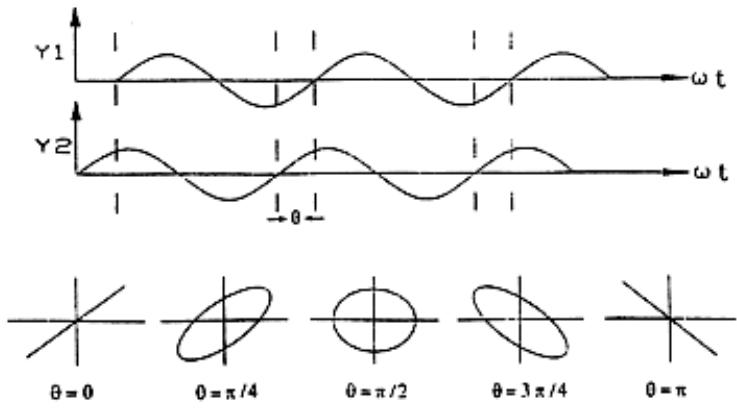
\includegraphics[keepaspectratio,alt={image}]{images/337738924ff11c35684b4db705985907d764b929c2740ede8dbf1c72e95c3095.jpg}}

图3 用李萨如图观察相位变化

\subsection{5.
时差法测量原理}\label{ux65f6ux5deeux6cd5ux6d4bux91cfux539fux7406}

连续波经脉冲调制后由发射换能器发射至被测介质中，声波在介质中传播，经过
t时间后，到达L距离处的接收换能器。由运动定律可知，声波在介质中传播的速度可由以下公式求出：速度V=距离L/时间t

\pandocbounded{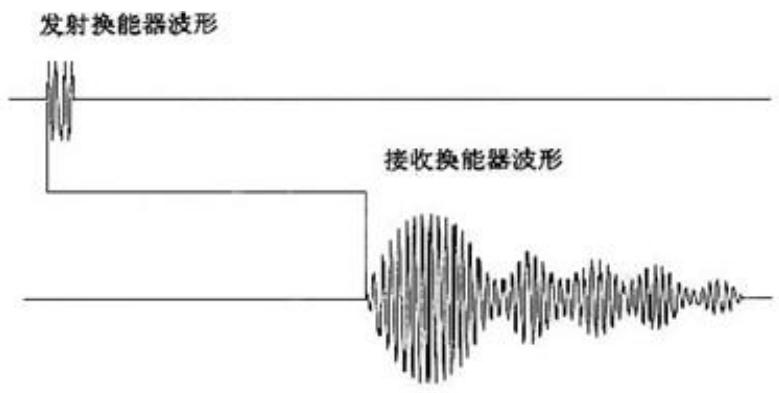
\includegraphics[keepaspectratio,alt={image}]{images/05a4f1d88a9c23650d0ace8832badc6ffc358608fadfefec55bc12b01025de47.jpg}}

图4 发射波与接收波

通过测量二换能器发射接收平面之间距离 L 和时间 t
,就可以计算出当前介质下的声波传播速度。

\subsection{四、实验内容：}\label{ux56dbux5b9eux9a8cux5185ux5bb9}

\subsection{1. 仪器预热：}\label{ux4eeaux5668ux9884ux70ed}

仪器在使用之前，加电开机预热
15min。在接通市电后，自动工作在连续波方式，这时脉冲波强度选择按钮不起作用。

\subsection{2.
驻波法测量声速：}\label{ux9a7bux6ce2ux6cd5ux6d4bux91cfux58f0ux901f}

\subsection{2.1
测量装置的连接}\label{ux6d4bux91cfux88c5ux7f6eux7684ux8fdeux63a5}

如图5所示，信号源面板上的发射端换能器接口（S1），用于输出一定频率的功率信号，请接至测试架的发射换能器（S1）；信号源面板上的发射端的发射波形Y1，请接至双踪示波器的
CH1（Y1），用于观察发射波形；接收换能器（S2）的输出接至示波器的
CH2（Y2），用于观察换能器接收波形。

\pandocbounded{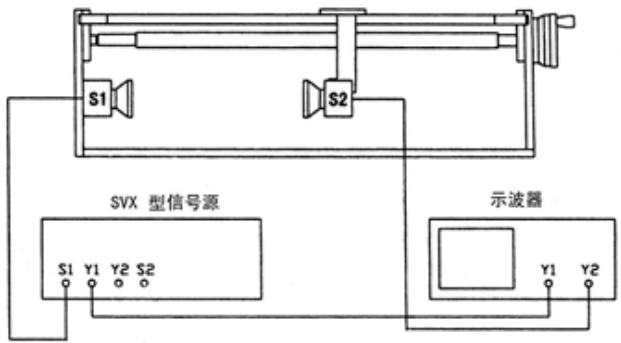
\includegraphics[keepaspectratio,alt={image}]{images/607a98db9b71d9ab149ead4c1f427797c0a36c3e99bd6f682a059a77db526c73.jpg}}

图5 驻波法、相位法连线图

\subsection{2.2
测定压电陶瓷换能器的测试频率工作点}\label{ux6d4bux5b9aux538bux7535ux9676ux74f7ux6362ux80fdux5668ux7684ux6d4bux8bd5ux9891ux7387ux5de5ux4f5cux70b9}

只有当换能器 S1 的发射面和 S2
的接收面保持平行时才有较好的接收效果。为了得到较清晰的接收波形，应将外加的驱动信号频率调节到换能器
S1、S2的谐振频率处时，才能较好的进行声能与电能的相互转换（实际上有一个小的通频带），S2才会有一定幅度的电信号输出，才能有较好的实验效果。

换能器工作状态的调节方法如下：首先调节发射强度旋钮，使声速测定仪信号源输出合适的电压，再调整信号频率（在
～ 之间），观察频率调整时 （
）通道的电压幅度变化。合适选择示波器的扫描时基 t/div
和通道增益，并进行调节，使示波器显示稳定的接收波形。在某一频率点处（34～40kHz
之间），电压幅度明显增大，再适当调节示波器通道增益，仔细地细调频率，使该电压幅度为极大值，此频率即是压电换能器相匹配的一个谐振工作点，记录频率
\(\mathrm { F _ { N } } .\) 。改变 和
间的距离，适当选择位置，重新调整，再次测定工作频率，共测5次，取平均频率
f。

在一定的条件下，不同频率的声波在介质中的传播速度是相等的。利用换能器的不同谐振频率的谐振点，可以在用一个谐振频率测量完声速后，再用另外一个谐振频率来测量声速，就可以验证以上结论。

\subsection{2.3 测量步骤}\label{ux6d4bux91cfux6b65ux9aa4}

将测试方法设置到连续波方式，选择合适的发射强度。完成前述 2.1 和 2.2
步骤后，选好谐振频率。然后转动距离调节鼓轮，这时波形的幅度会发生变化，记录下幅度为最大时的距离
\(\mathrm { L } _ { \mathrm { i } - 1 }\)
，距离在机械刻度上读出。再向前或者向后（必须是一个方向）移动距离，当接收波经变小后再到最大时，记录下此时的距离
\(\mathrm { L } _ { \mathrm { i } } \mathrm { _ { c } }\)
。即可求得声波波长：
\(\lambda _ { \mathrm { i } } { = } 2 \left| \mathrm { L } _ { \mathrm { i } } { - } \mathrm { L } _ { \mathrm { i } - 1 } \right|\)
。多次测定，用逐差法处理数据。

\subsection{3.
相位法/李萨如图法测量声速：}\label{ux76f8ux4f4dux6cd5ux674eux8428ux5982ux56feux6cd5ux6d4bux91cfux58f0ux901f}

将测试方法设置到连续波方式，选择合适的发射强度。完成前述 和
步骤后，将示波器打到 \(^ { 6 6 } \mathrm { X - Y ^ { 5 } }\)
方式，选择合适的示波器通道增益，示波器显示李萨如图形。转动鼓轮，移动S2，使李萨如图显示的椭圆变为一定角度的一条斜线，记录下此时的距离
\(\mathrm { L } _ { \mathrm { i } - 1 }\)
，距离由机械刻度尺读出。再向前或者向后（必须是一个方向）移动距离，使观察到的波形又回到前面所说的特定角度的斜线，这时接收波的相位变化
2π，记录下此时的距离 \(\mathrm { L } _ { \mathrm { i } \circ }\)
。即可求得声波波长：
\(\lambda _ { \mathrm { i } } { = } \left| \mathrm { L } _ { \mathrm { i } } { - } \mathrm { L } _ { \mathrm { i } - 1 } \right|\)
。

注意：在干涉法/相位法测量数据处理时，已知波长
\(\lambda _ { \mathrm { i } }\)
和频率f（频率由声速测定仪信号源频率显示窗口直接读出）。则声速
\(\mathrm { C _ { i } { = } } \lambda _ { \mathrm { i } } { \times } \mathrm { f } _ { \mathrm { i } }\)
。因为，声速还与介质温度有关，所以必要时请记下介质温度t
\(( ^ { \circ } \mathrm { C } )\) C

\subsection{4.
时差法测量声速：}\label{ux65f6ux5deeux6cd5ux6d4bux91cfux58f0ux901f}

\pandocbounded{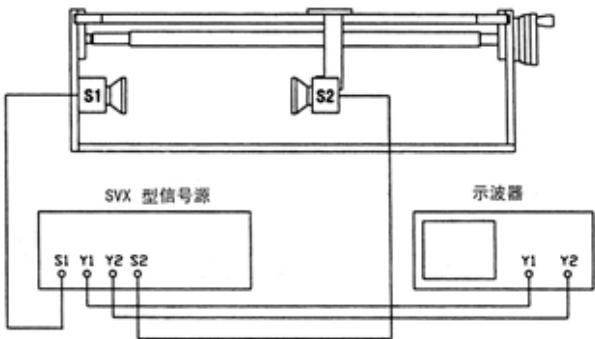
\includegraphics[keepaspectratio,alt={image}]{images/949dee6656d1d3847d162fbe7c2521f96ffb400f63c19417e720c0c11ef4d48a.jpg}}

图6 时差法测量声速接线图

使用空气为介质测试声速时，按图 6 所示进行接线，这时示波器的 Y1 和
Y2通道分别用于观察发射和接收波形。为了避免连续波可能带来的干扰，可以将连续波频率调离换能器谐振点。将测试方法设置到脉冲波方式，选择合适的脉冲发射强度。将S2移动到离开
S1一定距离（≥50mm），选择合适的接收增益，使显示的时间差值读数稳定。然后记录此时的距离值和信号源计时器显
\(\overline { { \overline { { \mathbf { \Omega } } } } }\) 的时间值
\(\mathrm { L } _ { \mathrm { i } - 1 }\) 和
\(\mathrm { t _ { i - 1 } } _ { \mathrm { ~ c ~ } }\) 。移动
S2，记录多次测量的距离值和显示的时间值
\(\mathrm { L } _ { \mathrm { i } }\) 和
\(\mathfrak { t } _ { \mathrm { i } \mathrm { c } }\) 。则声速
\(\scriptstyle \mathrm { C _ { i } = ( L _ { i } - L _ { i - 1 } ) / ( t _ { i } - t _ { i - 1 } ) }\)

\subsection{五、注意事项：}\label{ux4e94ux6ce8ux610fux4e8bux9879}

1．使用时，应避免声速测定仪信号源的功率输出端短路。

2．严禁将液体（水）滴到数显尺杆和数显表头内，如果不慎将液体（水）滴到数显尺杆和数显表头上，请用
\(6 0 \mathrm { { } ^ { \circ } C }\) 以下的温度将其烘干，即可使用。

3．若测试架体带有有机玻璃，容易破碎，使用时应谨慎，以防止发生意外。

\subsection{附录1
简析三种测试声速的方法}\label{ux9644ux5f551-ux7b80ux6790ux4e09ux79cdux6d4bux8bd5ux58f0ux901fux7684ux65b9ux6cd5}

\subsection{1.
驻波法（共振干涉法）}\label{ux9a7bux6ce2ux6cd5ux5171ux632fux5e72ux6d89ux6cd5}

由测试架上发射换能器发射出的声波经介质传播到接收换能器时，在接收换能器表面（是一个平面）产生反射。此时反射波与入射波在换能器表面叠加，叠加后的波形具有驻波特性。从声波理论可知，当二个声波幅度相同，方向相反进行传播时，在它们的相交处进行声波干涉现象，出现驻波。而声强在波幅处最小，在波节处最大。所以调节接收换能器的位置，通过示波器看到的波形幅度也随位置的变化而出现起伏，因为是靠目测幅度的变化来知道它的波长，所以难以得到很精确的结果。特别是在液体中传播，由于声波在液体中衰减较小，发射出的声波在很多因素影响下产生多次反射叠加，在接收换能器表面已经是多个回波的叠加（混响），叠加后的波形的驻波特征较为复杂，并不是根据单纯的两束波叠加来观察它的幅度变化，来求出波长。因此用通常的两束波叠加的公式来求速度，其精确性大为下降，导致测量结果不确定性的增大。通过在测试槽中的左、中、右三处进行测量，可以明确看出用通常的计算公式，在不同的地方计算得到的声速是不一样的。

\subsection{2.
相位比较法（李萨如图法）}\label{ux76f8ux4f4dux6bd4ux8f83ux6cd5ux674eux8428ux5982ux56feux6cd5}

声速在传播途中的各个点的相位是不同的，当发射点与接收点的距离变化时，二者的相位差也变化了。通过示波器用李萨如图法进行波长的测量。与驻波法相同的是都是目测波形的变化来求它的波长，同样测量结果存在着一定的不确定性。同样因为声波在液体中传播存在着多个回波的干涉影响，从而导致测量结果的不确定性的增大。

\subsection{3. 时差法}\label{ux65f6ux5deeux6cd5}

在实际工程中，时差法测量声速得到广泛的应用。时差法测试声速的基本原理是基于速度
距离 时间
，通过在已知的距离内计测声波传播的时间；从而计算出声波的传播速度，在一定的距离之间
由控制电路定时发出一个声脉冲波，经过一段距离的传播后到达接收换能器。接收到的信号经放大，滤波后由高精度计时电路求出声波从发出到接收这个在介质传播中经过的时间，从而计算出在某一介质中的传播速度。只因为不用目测的方法，而由仪器本身来计测，所以其测量精度相对于前面两种方法要高。同样在液体中传播时，由于只检测首先到达的声波的时间，而与其它回波无关，这样回波的影响比较小，因此测量的结果较为准确，所以工程中往往采用时差法来测量。

综上所述，通过分析三种测量方法，我们得出了用驻波法和相位法这两种方法测量声速，存在一定的视觉测量误差，建议学生带着比对、加深印象目的使用这三种方法进行测量声速，并对三种方法的优点、缺点进行比较。若课时允许，建议学生对水中用相位法、驻波法测量误差的原因，从声传播过程中混响现象出发展开讨论和分析，进一步了解声波在不同介质当中传播的知识。

\end{document}
